\documentclass[11pt,a4paper]{article}

% ---------- Packages ----------
\usepackage[a4paper,margin=2cm]{geometry}
\usepackage[utf8]{inputenc}
\usepackage[T5]{fontenc} % use [T5]{fontenc} (with the vietnam/vntex package) if you switch the report to Vietnamese
\usepackage{graphicx}
\usepackage{booktabs}
\usepackage{enumitem}
\usepackage{hyperref}
\usepackage{caption}
\usepackage{xcolor}
\usepackage{titlesec}
\usepackage{fancyhdr}
\usepackage{listings}

\hypersetup{
    colorlinks=true,
    linkcolor=blue,
    urlcolor=blue,
    citecolor=blue
}

\titlespacing*{\section}{0pt}{10pt}{6pt}
\titlespacing*{\subsection}{0pt}{8pt}{4pt}

\pagestyle{fancy}
\fancyhf{}
\fancyhead[L]{HCMC AI Challenge 2026 -- Technical Report}
\fancyhead[R]{\thepage}
\renewcommand{\headrulewidth}{0.4pt}

\hypersetup{
    colorlinks=true,
    urlcolor=blue
}

\title{\vspace{-1.5cm}\textbf{Technical Report} \\[4pt]
\large Ho Chi Minh City AI Challenge 2026 \\[2pt]
\large Determinatives}
\author{
    Bui Thien Nghia \\
    \small Vietnamese-German University
    \and
    Nguyen Ngoc Thanh Huong \\
    \small VNUHCM - University of Science
    \and
    Nguyen Tran Minh Khang \\
    \small VNUHCM - University of Science
    \and
    Thai Cao Nha \\
    \small Industrial University of Ho Chi Minh City
    \and
    To Ngoc Quynh Nhu \\
    \small VNUHCM - University of Science
}
\date{September 12th, 2026}

\begin{document}
\maketitle
\thispagestyle{fancy}
\vspace{-1cm}

% =========================================================
\section{Overview}

Our system is a multimodal, zero-shot, keyframe-based Video Moment Retrieval (VMR) pipeline built for the HCMC AI Challenge 2026. It is composed of a Python \texttt{BackEnd} that performs offline video preprocessing/indexing and exposes retrieval through a Django REST API, and a React/TypeScript \texttt{FrontEnd} that gives the team an interactive, cooperative retrieval and answer-submission workspace covering all three contest query types: KIS (Known-Item Search), QA (Question Answering) and TRAKE (multi-moment/temporal key-event retrieval).

The core retrieval idea is a tri-vector hybrid search over a single Qdrant collection (a SigLIP2 visual-semantic embedding, a BGE-M3 dense text embedding, and a BGE-M3 sparse lexical embedding, fused at query time) optionally followed by a temporal re-ranking stage that rewards keyframes sitting inside a locally coherent visual/temporal neighbourhood, which is a natural fit for moment retrieval rather than isolated frame retrieval. We aim to contribute an entirely local, lightweigt, multi-grained, retrieval framework coupled with an interactive, multi-purposed retrieval user interface.

Our project is accessible on GitHub at \url{https://shorturl.at/5AeWJ}

% =========================================================
\section{Strategy}

\subsection{System Architecture Overview}

\begin{figure}[h!]
    \centering
    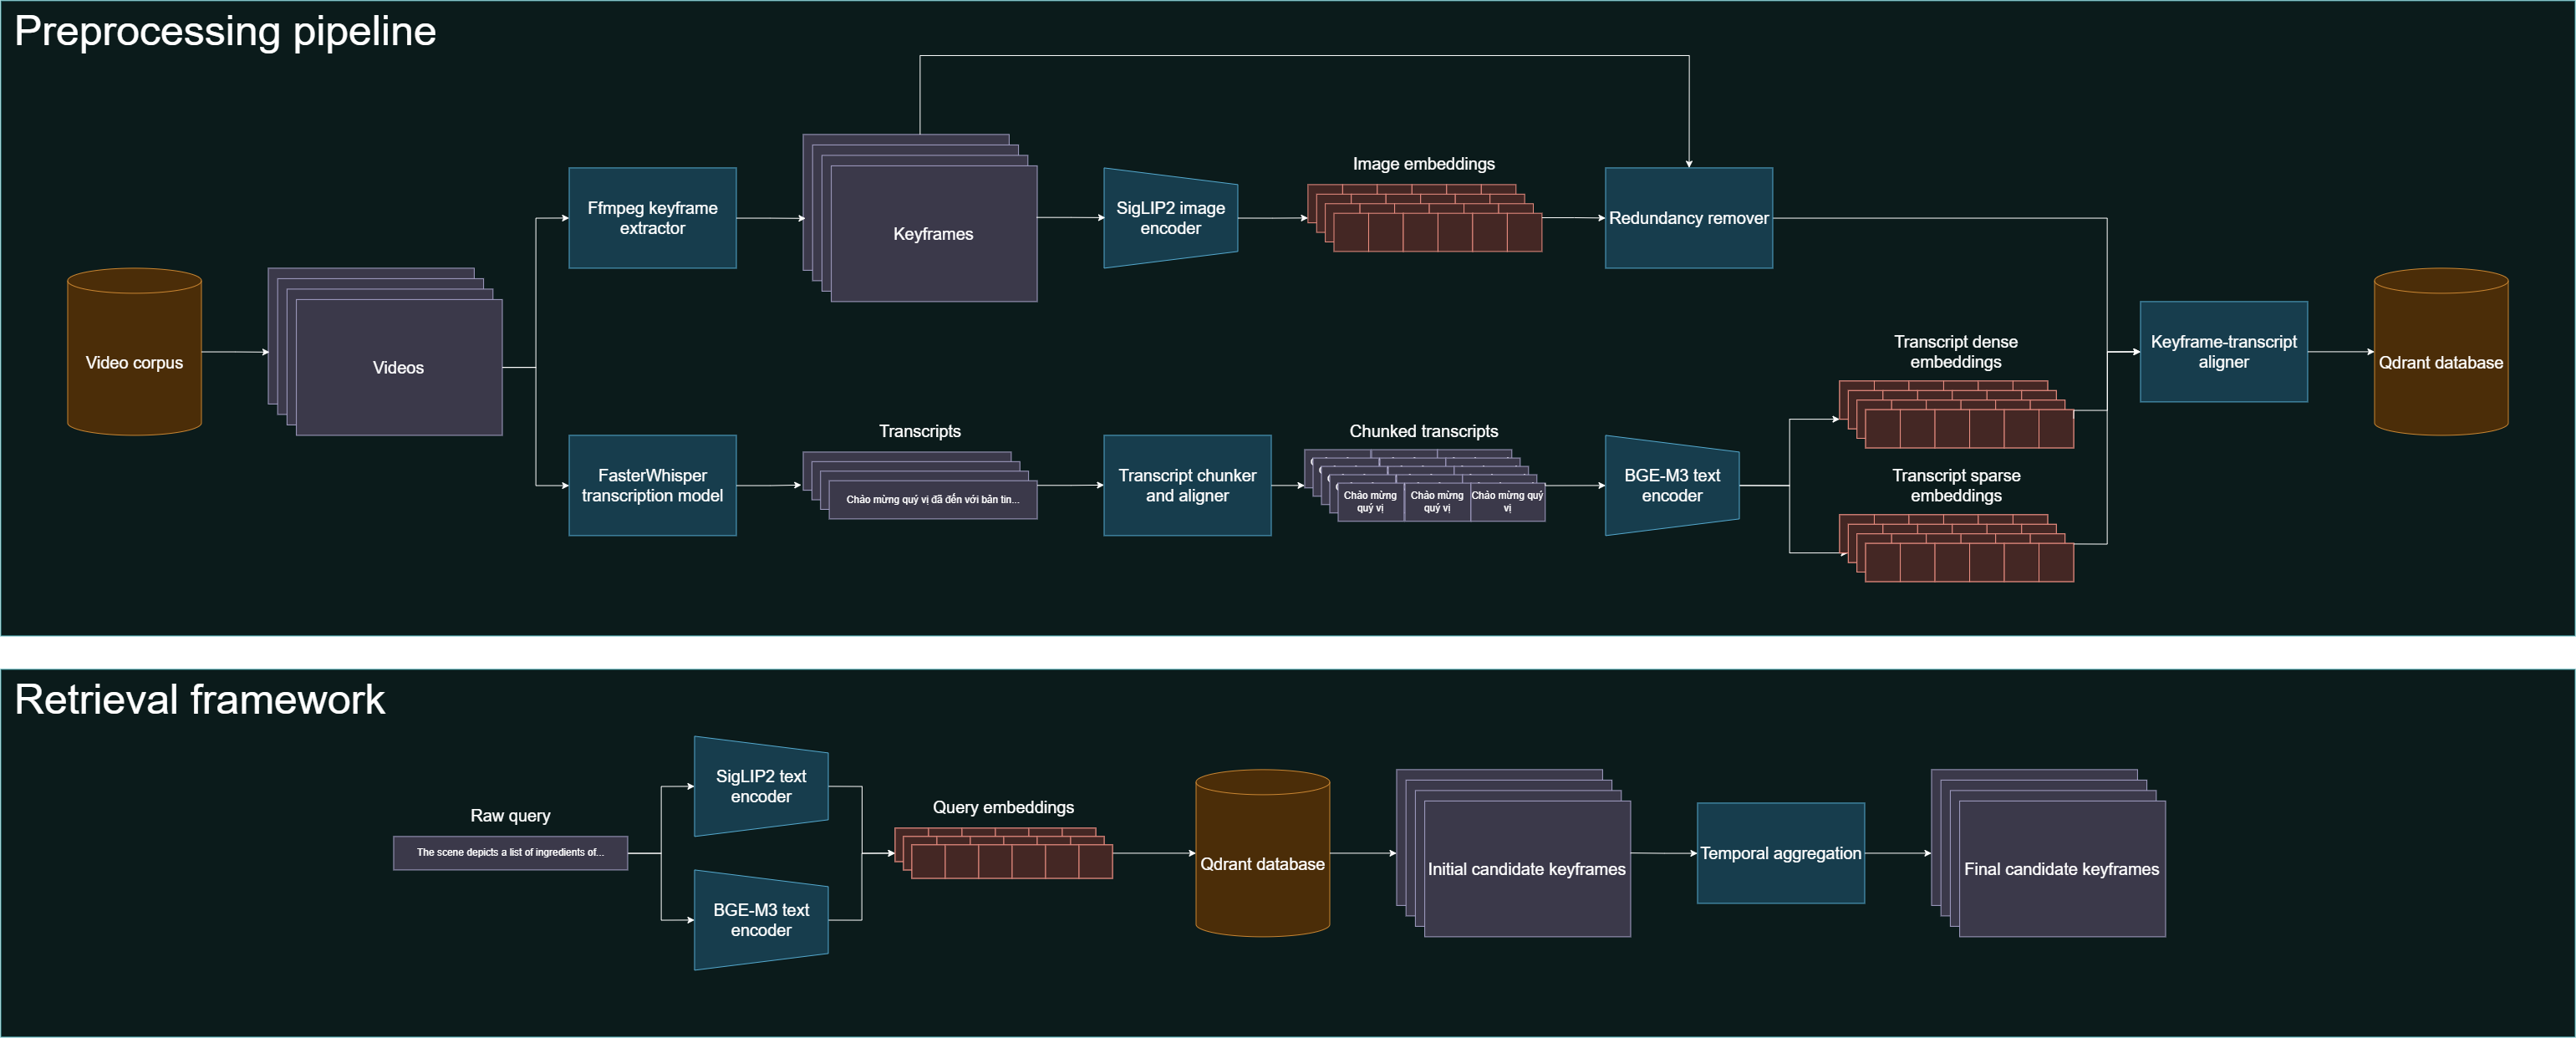
\includegraphics[width=0.9\textwidth]{images/architecture.png}
    \caption{Overall system architecture.}
    \label{fig:architecture}
\end{figure}

At a high level, the pipeline consists of two stages:
\begin{enumerate}[leftmargin=1.5em]
    \item \textbf{Offline data processing and indexing stage}: each video is decoded into representative keyframes and, in parallel, transcribed; every keyframe and transcript chunk is embedded into three shared vector spaces and upserted into a Qdrant collection as a single point with multiple named vectors plus rich metadata payload.
    \item \textbf{Online query stage}: a free-text query typed into the FrontEnd is sent to the Django REST API, encoded into the same three vector spaces, fused/searched (and optionally re-ranked) against the Qdrant index, and the ranked keyframes are streamed back to the results grid for the team to inspect and submit.
\end{enumerate}

\subsection{Data Preprocessing}
\subsubsection{Visual Data Extraction}
Keyframes are extracted per-video with FFmpeg's shot detector: frames are selected when the frame-to-frame scene score exceeds a \texttt{shot\_confidence\_score} threshold and at least \texttt{min\_keyframe\_distance} seconds have passed since the previous selected frame, which prevents over-segmenting near-static shots while maintaining sufficient temporal granularity. Each keyframe is tagged with its frame index, frame order (absolute frame number), timestamp, the video's FPS, and then encoded with SigLIP2 into a shared image-text embedding space.

Because scene-change detection can still emit visually near-identical frames (e.g. slow pans, static talking-head shots), extracted keyframes are de-duplicated with agglomerative clustering on their SigLIP2 embeddings. Only the frame closest to each cluster's centroid is kept, which keeps the index compact without losing visually distinct moments.

\subsubsection{Aural Data Extraction}
Audio is transcribed with a batched Faster-Whisper pipeline with a word-level output configuration. The output, which is a list of words, their start and end timestamps, is then grouped into sentence-like chunks by punctuation boundaries or a maximum duration cap. Each keyframe is then aligned to the transcript chunks falling inside a symmetric \texttt{alignment\_transcript\_time\_range} window with the center being its own timestamp, giving every keyframe a local speech-context string. Transcript chunks are embedded with BGE-M3 into both a dense semantic vector and a sparse lexical (token-weight) vector.

\subsubsection{Packaging and Storage}
Per-keyframe features (SigLIP2 dense, BGE-M3 dense, BGE-M3 sparse token ids/weights) are compacted into a single \texttt{.npz} per keyframe, and per-video metadata (frame id, frame order, timestamp, fps, aligned transcript, source link) is consolidated into per-video CSV maps that are later merged into the Qdrant payload for each point.

Regarding the Qdrant database, its schema is described as follows:

\begin{lstlisting}
    {
        "vectors": {
            "siglip2_dense": {
                "size": 1536,
                "distance": "Cosine",
            },
            "bgem3_dense": {
                "size": 1024,
                "distance": "Cosine",
            },
            "bgem3_sparse": {
                "distance": "Dot",
                "modifier": "idf"
            }
        },
        "payload": {
            "frame_id": "keyword (Indexed)",
            "vid_id": "keyword (Indexed)",
            "frame_order": "integer (Indexed)",
            "time_order": "float (Indexed)",
            "fps": "float",
            "transcript": "text (Indexed)",
            "frame_path": "keyword",
            "vid_path": "keyword",
            "yt_link": "keyword"
        }
    }
\end{lstlisting}

\subsection{Retrieval Method}

\subsubsection{Query Processing}

Since the system performs zero-shot retrieval, no query-specific fine-tuning happens at contest time. A raw text query typed in the Search Panel is sent as-is to the backend and encoded directly into the collection's embedding spaces: the SigLIP2 text tower produces the visual-space query vector, and BGE-M3 produces the dense and sparse text-space query vectors from the same string. Because SigLIP2 and BGE-M3 are natively multilingual, the same code path can accept Vietnamese or English queries without an explicit translation step.

Aside from textual query, the system supports reusing already encoded keyframes as queries. Specifically, the vector set associated with a query keyframe is used to search against the Qdrant index to find other contextually (either in visual or aural terms) similar frames. This feature is specifically useful when one would like to reassess the correctness of their result by comparing it with its similar peers.

\subsubsection{Similarity Search}

All three vector types use cosine similarity. The dense collections are indexed with HNSW and INT8 scalar quantization for fast approximate top-k retrieval at contest scale; the sparse vector uses Qdrant's native sparse index. Structured payload fields (comprising \texttt{frame\_id}, \texttt{vid\_id}, \texttt{frame\_order}, \texttt{time\_order}, and a multilingual full-text \texttt{transcript} index) are indexed separately to support fast filtering.

\subsubsection{Ranking, Filtering, and Result Fusion}

Our retrieval method revolves around three search modalities: Visual (SigLIP2 only), Textual (BGE-M3 dense + sparse), and Hybrid (all three). These modalities are combined and used in 2 methods described below:

\begin{itemize}[leftmargin=1.5em]
    \item \textbf{Fast}: each active vector space is queried in parallel, and the candidate lists are fused with Reciprocal Rank Fusion (RRF) into a single ranked list. This is the default, low-latency path used for most searches during a round, allowing one to switch between modalities with ease based on the characteristics of the query.
    \item \textbf{Deep}: starts from a DBSF-fused candidate list, then re-ranks it with a temporal aggregation step. Specifically, for every candidate keyframe, its local neighbourhood within the same video (either its k nearest visual neighbours or all frames inside a time-distance window) is collected; each neighbour is weighted by a Gaussian temporal-decay kernel over its time distance to the candidate (whose bandwidth currently estimated robustly from the neighbourhood's first-quantile absolute deviation) combined with its own similarity to the query (a weighted blend of SigLIP2, BGE-M3 dense and BGE-M3 sparse similarity). This yields a temporal coherence score, complemented by a visual coherence bonus (currently a Shannon-entropy-based concentration measure), resulting in an aggregated score. The orignal and aggregated scores are normalized and linearly combined with the initial fused score to produce the final ranking. The overall formula for the final score of a candidate keyframe is describe as below:
    $$S_c = \frac{1}{|N|} \cdot \Sigma_{n \in N} (sim(n, q) \cdot RBF(|t_n, t_c|)) \cdot (1 - \frac{H(sim(N, c))}{ln(|N|)})$$
    where $c$ is the candidate keyframe; $N$ is the ANN keyframes list of frame $c$; $q$ is the query; $sim(\cdot)$ denotes the similarity calculation; $H(\cdot)$ denotes the Shannon entropy function; and $RBF(\cdot)$ denotes the Radial Basis Function decay kernel. Intuitively, Deep mode rewards keyframes that sit inside a temporally and visually coherent moment in the video, rather than isolated one-off matches. This provides the query a view of compacted candidate scenes as a whole, matching the characteristic of Video Moment Retrieval. Although modalities switching is not supported for this method and it is more time-consuming than the traditional ensemble search, it proves relative effectiveness in several complex, context-specific queries.
\end{itemize}

In addition to ranking methods, the Search Panel exposes schema-driven structured filters: ranges on \texttt{frame\_id}, \texttt{frame\_order}, \texttt{time\_order}, \texttt{transcript} full-text match, \texttt{vid\_id}, and any other indexed payload field the current collection reports, which are translated into Qdrant field conditions and can be combined with a text query or used separately for filter-based browsing.

% =========================================================
\section{User Interface}

The FrontEnd (React + TypeScript + Vite, Zustand for state, Tailwind for styling) is designed to support a multi-purpose and cooperative retrieval workflow, allowing multiple team members to search, inspect, and submit results collaboratively during a contest round.

\subsection{Overall Interface}

\begin{figure}[h!]
    \centering
    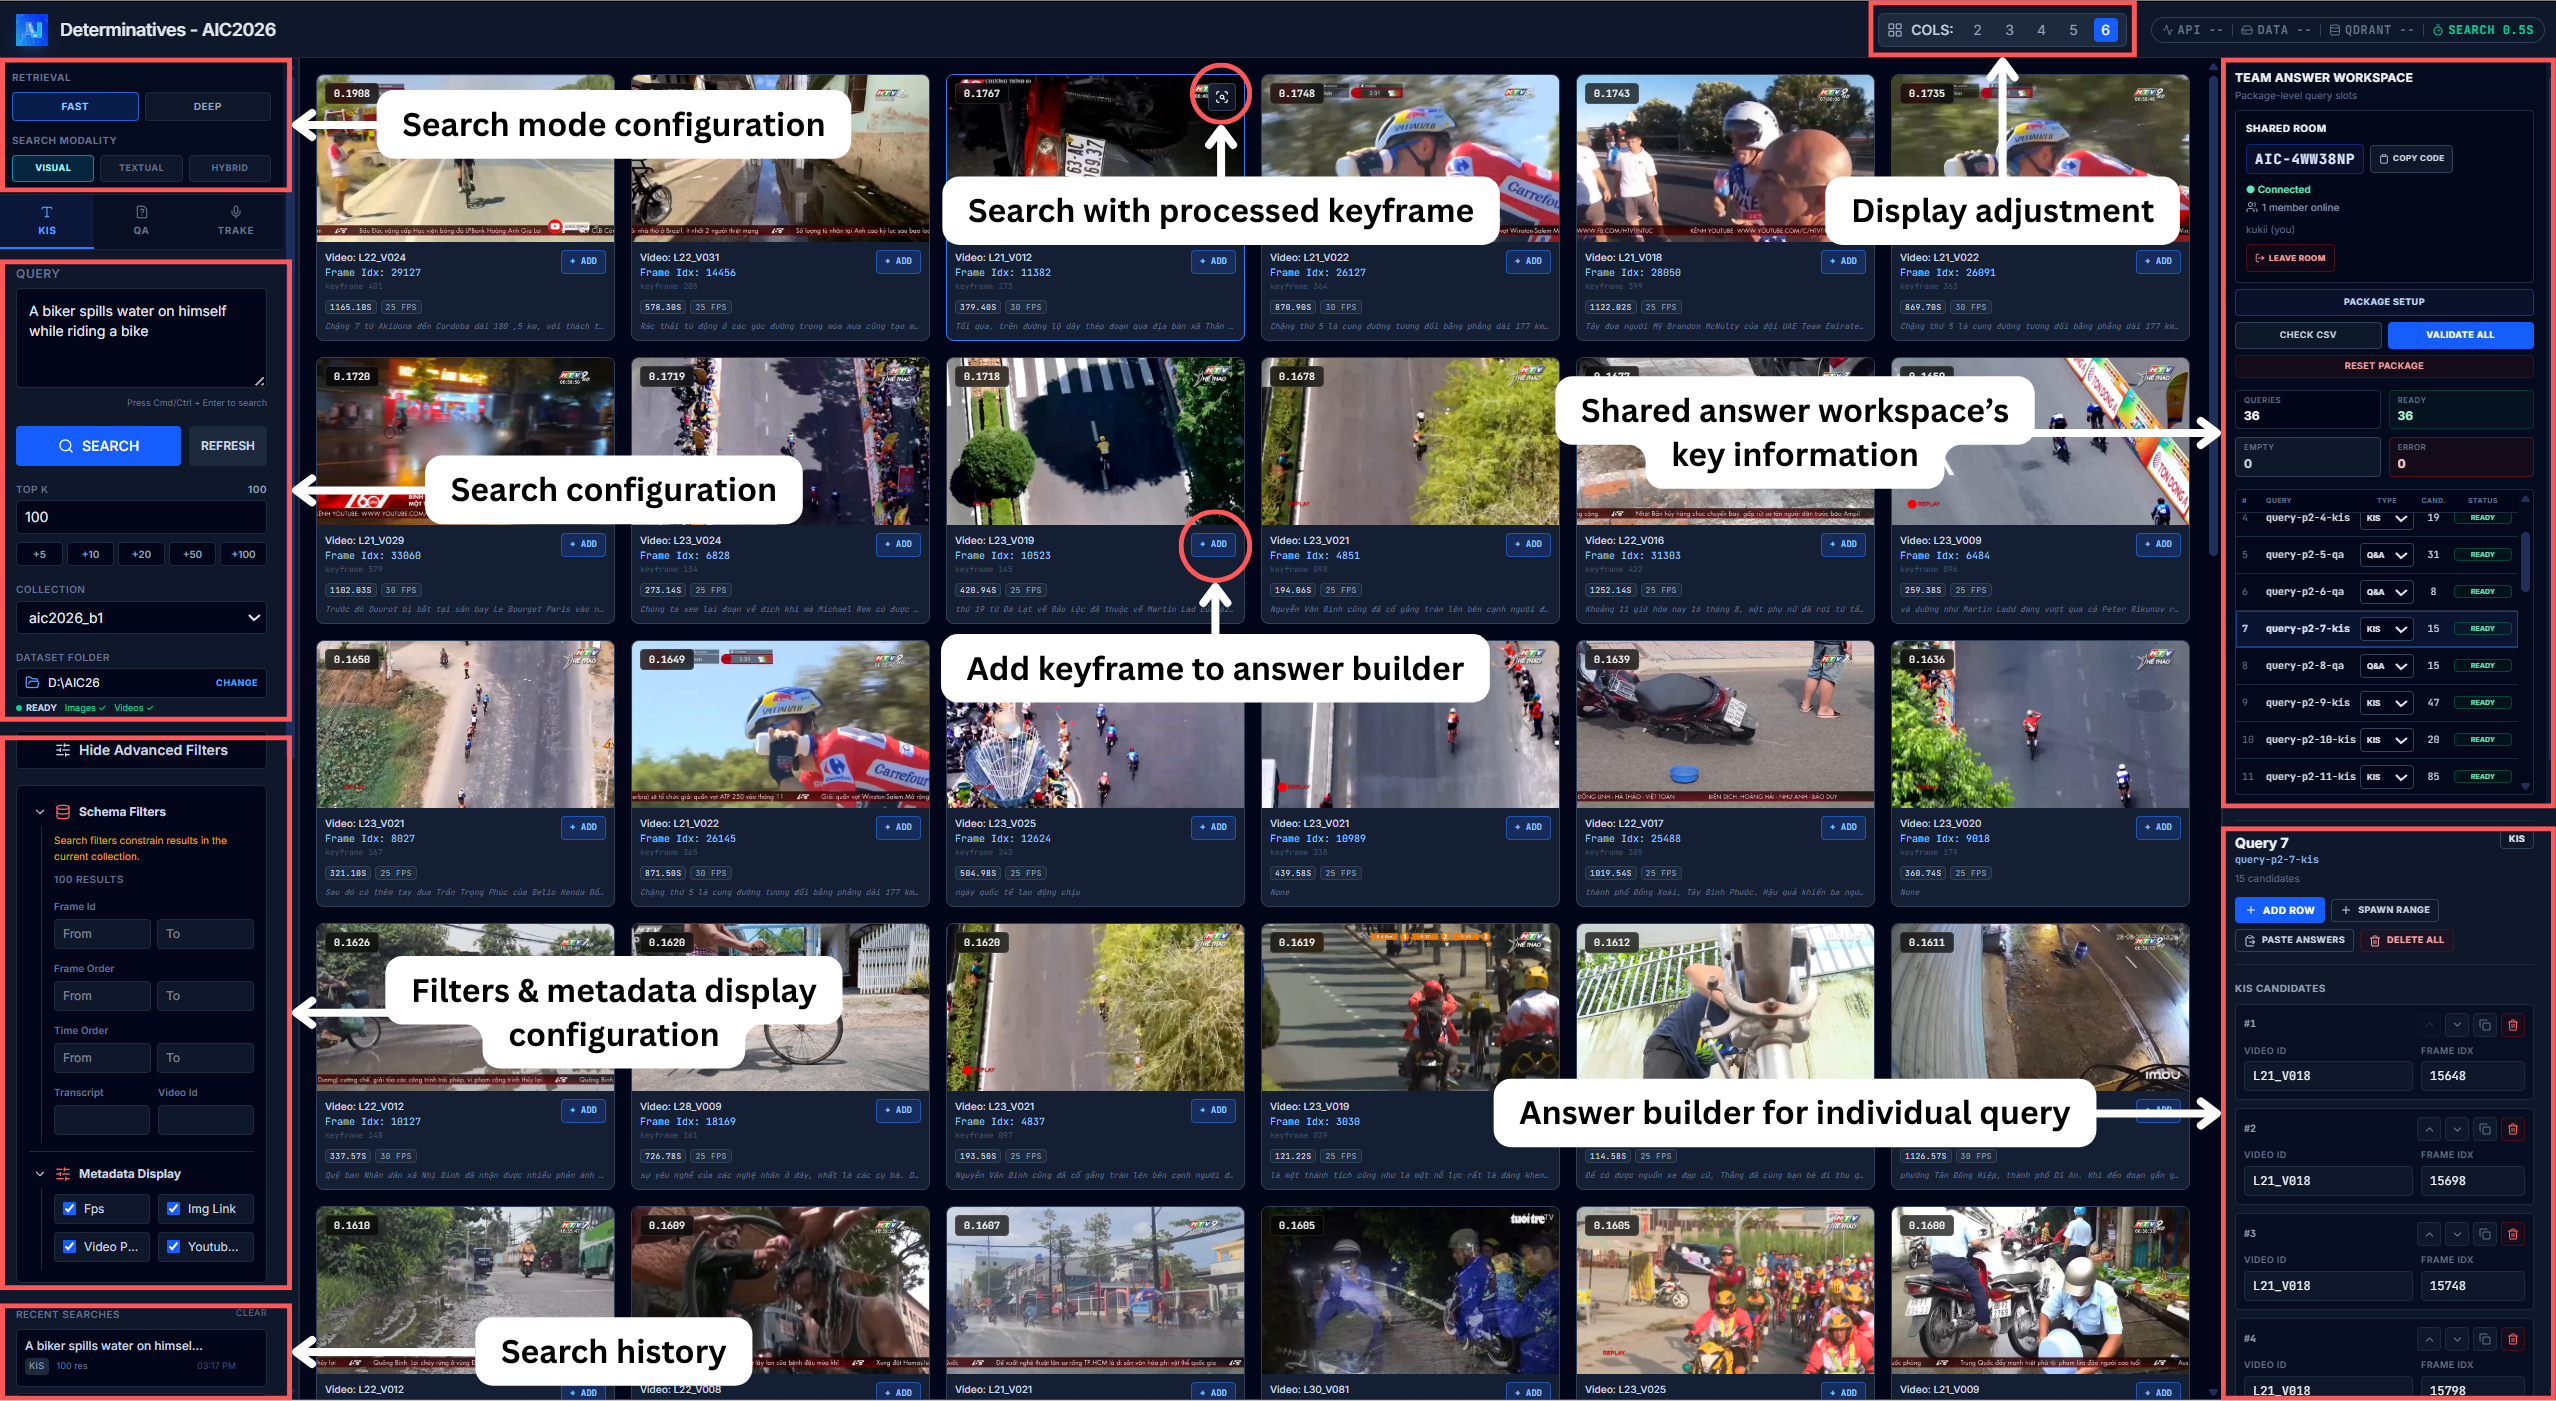
\includegraphics[width=0.95\textwidth]{images/ui_overall.png}
    \caption{Overall layout of the user interface}
    \label{fig:ui-overall}
\end{figure}

The app is a single-page, three-pane layout: a header bar (team logo, a 2-6 column density toggle for the results grid, and a live backend/collection status indicator) sits above a left search panel, a centre display panel (the result grid), and a right answer builder (the recheck / submission panel). The cooperative aspect is built inside the answer builder as a team room: any teammate can create a room and share a short room code. Everyone who joins shares one live submission package with a visible sync status (connected/syncing/offline/conflict) and built-in conflict resolution, so KIS/QA/TRAKE answers assembled by different teammates on different machines merge into a single package before export.

\subsection{Search Panel}

From top to bottom, the Search Panel offers: a retrieval toggle; a search modality toggle; a multi-line query textbox; a top-k control; a dataset/collection picker that auto-loads the collection's indexed payload schema; a collapsible filters section built dynamically from that schema; a metadata display toggle section for result cards; and a  history that can be restored or re-run with one click. The query type selection between the modality selection and query textbox is deprecated due to incompatibility with our current answer builder's version, but was not removed.

\subsection{Display Panel}

\begin{figure}[h!]
    \centering
    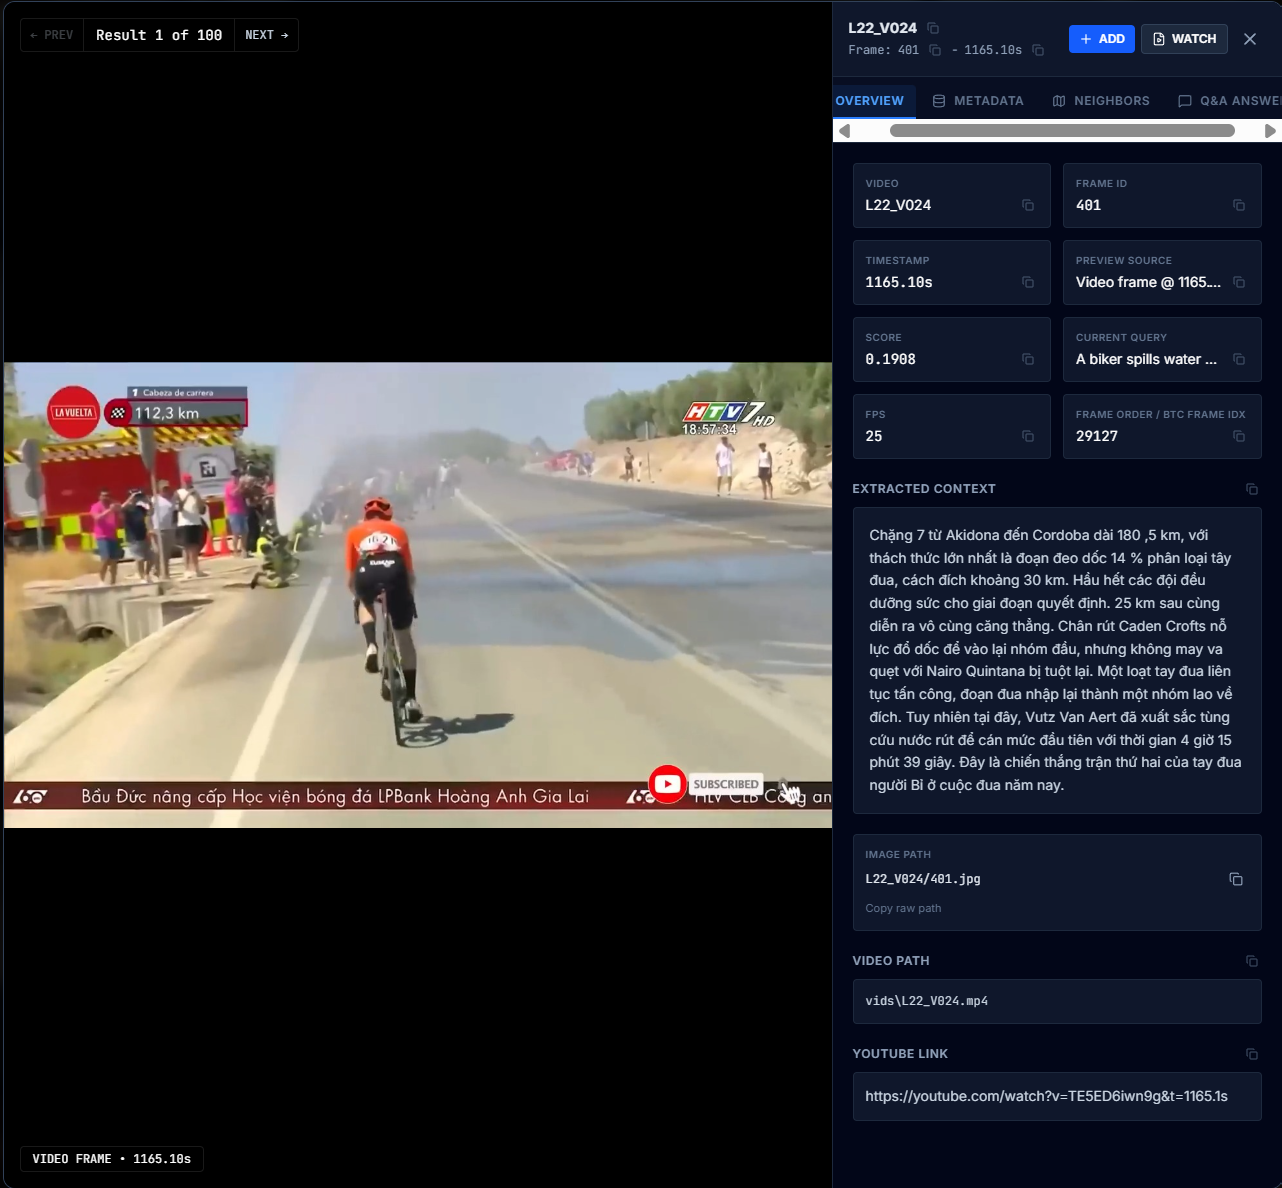
\includegraphics[width=0.8\textwidth]{images/preview.png}
    \caption{A preview pop-up of a candidate keyframe}
    \label{fig:inspection}
\end{figure}

\begin{figure}[h!]
    \centering
    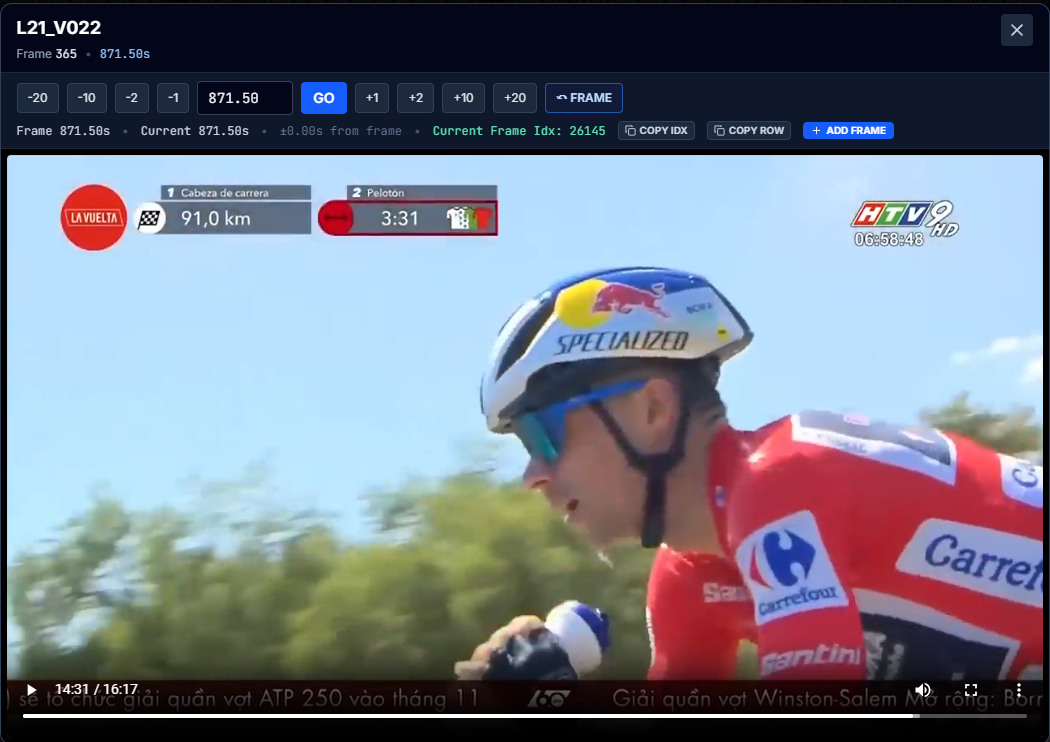
\includegraphics[width=0.8\textwidth]{images/inspection.png}
    \caption{A pop-up of a candidate keyframe for deep inspection}
    \label{fig:preview}
\end{figure}

Results render as a responsive, lazily-loaded grid (2-6 columns, configurable from the header). Each card shows the matched keyframe, its similarity score, video id, frame index/timestamp, FPS, and a truncated transcript snippet; cards are draggable and expose two inline actions: "Search from this frame" (query-by-example) and "+ Add" (send straight to the active Answer Builder query). Clicking a card opens a preview modal with the full-resolution keyframe, its neighbouring keyframes for quick temporal context, and the complete metadata payload; From the preview modal, a video modal can play the source video starting at the matched timestamp, with frame-accurate stepping and in-video frame capture for fine-tuning the exact submitted frame.

\subsection{Answer Builder}

\begin{figure}[h!]
    \centering
    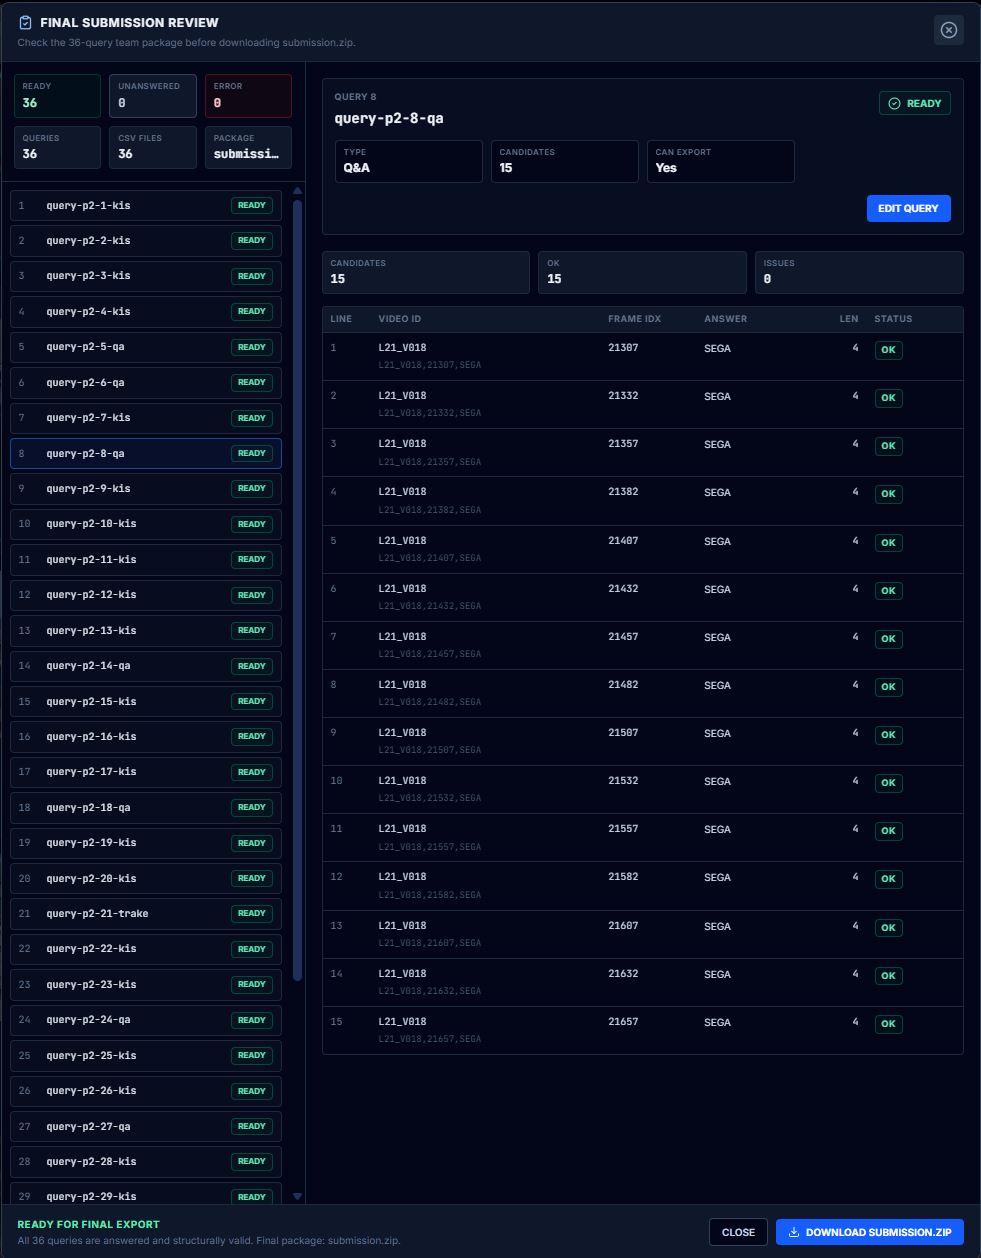
\includegraphics[width=0.8\textwidth]{images/ans_review.png}
    \caption{The validation pop-up of the answer builder}
    \label{fig:ans-review}
\end{figure}

The Answer Builder adapts to the active query type:
\begin{itemize}[leftmargin=1.5em]
    \item \textbf{KIS} -- a drag-to-reorder ranked list of single-frame candidates, with automatic exact-duplicate and near-duplicate (frames within 30 indices of each other in the same video) warnings.
    \item \textbf{QA} -- the same ranked candidate list, plus a required free-text answer per candidate (with a length limit and validation), and an "apply this answer to every candidate from the same video" shortcut.
    \item \textbf{TRAKE} -- an ordered sequence of up to 20 timestamped events within a single video, built and reordered directly from search results.
\end{itemize}
All three feed into a submission workspace that can hold several named queries at once, supports pasting/importing answers from CSV, runs a final validation/review pass before export, and downloads the package as CSV/zip files following the contest's required naming convention, synchronized live across the team through the Team Room described above. To ensure correctness, keyframes of an entire scene can be added to an individual query by using the "spawn range" utility: one types the answer's video, start and end frame indices or timestamps of the scene, and the distance between each frame, and the system automatically formulates a list of answer keyframes from the scene.

% =========================================================
\section{Case Study}

During our participation in the 21/08, 28/08, and 04/09 preliminary rounds, we have encountered multiple issues in finding and validating the answers. Consequently, we carried out several in-depth inspections and reviews, resulting in findings generalized as follows:

\subsection{Case 1: queries requiring recognition of sequence and camera angles}

\begin{quote}
    ``Cảnh phim lần lượt giới thiệu các nguyên liệu của món ăn qua 3 chuyển cảnh: máy quay chéo lên và kết thúc ở nguyên liệu hải sản đầu tiên; quay từ trên xuống cận cảnh nguyên liệu hải sản thứ hai rồi chuyển sang các nguyên liệu nhiều màu sắc; cuối cùng là cú máy tĩnh toàn cảnh toàn bộ nguyên liệu.''
\end{quote}

The system is capable of retrieving keyframes that are visually similar to the described content. However, to accurately identify the target scene, the team still needs to watch the video and pay attention to the sequence of transitions and camera angles. This is a challenging aspect of the query because individual keyframes may be visually similar in terms of content but cannot fully represent the relationships between the sequence of events and camera movements. Through this scenario, the team found that queries describing image sequences, camera angles, and transitions between scenes require greater precision and stronger temporal-context analysis than queries that only identify a single image.

\subsection{Case 2: queries with multiple similar segments}

\begin{quote}
    ``Trong một ngôi nhà nông thôn có cửa sổ lớn, hai người phụ nữ đang làm thủ công trên một bộ ván ngựa, phía sau là một dãy khoảng 10 thớt gỗ được treo thành một hàng ngang.''
\end{quote}

The system returns keyframes that accurately match the description. However, multiple segments in the video contain keyframes similar to the query, making it difficult to determine the exact moment requested by the Organizing Committee. The team initially used the conventional query approach, through which the system returned multiple relevant keyframes belonging to different segments. Although these results helped narrow down the search space, the system was still unable to accurately identify the exact keyframe requested by the Organizing Committee.

Through this scenario, the team found that providing additional distinctive and specific details in the query can help narrow the search space, improve the system's ability to distinguish between similar segments, and increase the accuracy of identifying the target moment.

\subsection{Case 3: queries with correct content but incorrect timing}

\begin{quote}
    ``Câu hỏi môn Sinh học nằm ở số thứ tự 11 trong đề thi THPTQG 2022. Trong câu hỏi có một biểu đồ đưa ra sự so sánh tốc độ sinh trưởng của các loài thực vật trong các hệ sinh thái ven biển. Hãy cho biết loài cây (II) đạt được tốc độ sinh trưởng tốt nhất khi môi trường sống có độ mặn là bao nhiêu phần nghìn?''
\end{quote}

Although the system returns a keyframe containing the correct content in the graph, it does not guarantee the correct timestamp. Specifically, the returned keyframe belongs to a video from 2024 rather than 2022 as required.

Accurately identifying both the content and the corresponding time still depends significantly on watching and listening to the video. This demonstrates that the system's temporal retrieval capability remains limited, particularly when similar content appears at multiple points in different videos or at different times. The team found that the system needs to improve its ability to retrieve and extract information from audio, while also integrating visual and audio information to improve the accuracy of identifying both the target content and the exact moment.


\subsection{Case 4: queries containing small and presumably insignificant visual details}

\begin{quote}
    ``Đoạn phim quay từ phía sau nhóm dẫn đầu, gồm 1 tay đua dẫn trước và 3 tay đua bám phía sau, khi cả nhóm rẽ phải vào đường Hồ Tùng Mậu tại giao lộ có đèn xanh đang đếm ngược đến 13 giây.''
\end{quote}

The system correctly identifies the main content as a group of cyclists. However, small but decisive details, such as the street name and the number of seconds displayed on the traffic light, are often overlooked or difficult to recognize accurately.

In particular, the information “Ho Tung Mau Street,” which is mentioned in the commentary, cannot currently be effectively exploited because of the system's limitations in audio-based retrieval mentioned above. In addition, the detail “at an intersection where the green traffic light is counting down to 13 seconds” is a small visual detail that appears only briefly in the video and is therefore difficult to identify from a keyframe.

As a result, the team had to review multiple videos and verify both visual and audio information across nearly all videos for which the system returned relevant keyframes. Through this scenario, the team found that the system needs to improve its ability to recognize small visual details in order to reduce the time required to locate a specific moment.

\subsection{Case 5: query optimization using distinctive details}

\begin{quote}
    ``Cảnh quay một chú lân đang biểu diễn từ đầu video, các cột để chú lân biểu diễn được dán những con số. Phía sau có 1 mô hình con rồng uốn lượn hình xoắn ốc. Trong các số từ 16 giây đầu tiên của video, số nào không được nhìn thấy từ góc nhìn của camera trong các số từ 1-8.''
\end{quote}

The answer to the question was compiled and inferred based on the results returned by the system. However, the team could not accurately identify the exact video and keyframe requested by the Organizing Committee. The main reason was that the query contained general information but lacked sufficiently distinctive details.

Therefore, more specific characteristics should be added, such as colors, object positions, distinctive object features, or details of the ongoing activity. These pieces of information serve as distinguishing cues between different videos, helping narrow the search space and increasing the likelihood of accurately retrieving the target content.

\begin{quote}
    ``Cảnh quay liệt kê các nguyên liệu để nấu một món ăn. Ảnh nền bao gồm dĩa thịt, bó lá tươi xanh đặt ở góc bên trái, một gói hạt nêm, hũ thủy tinh nhỏ đựng nước cốt dừa, bột cà ri, nấm mèo (mộc nhĩ) khô đặt phía dưới chén gia vị, sả cây và ớt hiểm đỏ đặt ở góc trái phía dưới. Bảng nguyên liệu hiện lên gồm 9 thành phần cụ thể. Hỏi phần thịt có trọng lượng bao nhiêu trong bảng nguyên liệu (số và đơn vị được ghi trong bảng)?''
\end{quote}

The query describes many details of the scene, including the ingredients and their positions. When all of this information is used in the query, the system returns a broad range of results, including many videos that contain only some of the described ingredients while also showing additional ingredients.

When querying for “wood ear mushrooms,” the returned results still include images of wood ear mushrooms that do not contain the exact answer. However, the search scope becomes narrower and easier to verify.

The team found that selecting distinctive and less frequently occurring details, such as “wood ear mushrooms,” helps the system focus on the specific object of interest. In contrast, including too many objects in a query makes it more difficult for the system to determine which object should be prioritized and causes the result space to become broader.

Through these two scenarios, the team found that including all available information in a query does not always produce the most effective results. Instead, selecting or adding highly distinctive details has a direct impact on both the search scope and the accuracy of retrieval results. This requires users to carefully observe the scene and select highly discriminative features when constructing an effective query.

% =========================================================
\section{Conclusion}

Our team introduces a tri-vector retrieval solution with novel temporal re-ranking, as well as an interactive user that both supports a wide range of tasks and facilitates teamwork. After the preliminary round, our greatest limitations remain the aggregation method, the inconspicuous visual and aural cues, and the team's retrieval skill, as shown by the query analysis. We plan to improve our embedding fusion method, overhaul the current preprocessing pipeline, and upgrade towards a multi-grained retrieval framework. If possible, we will consider adding more advanced retrieval methods such as query preprocessing and answer hinting in the near future.

\end{document}
